% =============================================================
% 4.1 การออกแบบเนื้อเรื่องของเกม (Storyboard)
% โครงงาน: การออกแบบและพัฒนาเกมเดินเรือด้วยระบบสั่งการด้วยเสียงเพื่อส่งเสริมทักษะการสื่อสาร
% =============================================================

\section{การออกแบบเนื้อเรื่องของเกม (Storyboard)}

ผู้เล่นจะได้สวมบทบาทเป็น \textbf{``กัปตันเรือ''} (Captain) ผู้รับผิดชอบในการนำเรือบรรทุกสินค้าเดินทางฝ่าน่านน้ำที่เต็มไปด้วยอุปสรรคและความท้าทาย โดยเนื้อเรื่องจะสะท้อนถึงการฝึกฝนทักษะการสื่อสารภาษาอังกฤษและการตัดสินใจภายใต้สถานการณ์กดดัน ผ่านการสั่งการลูกเรือปัญญาประดิษฐ์ (AI Crew) ได้แก่ พลต้นหน (Navigator) และพลถือท้าย (Helmsman) ลำดับเหตุการณ์และเนื้อเรื่องภายในเกมแสดงดังตารางที่ \ref{tab:storyboard}

\begin{table}[H]
\centering
\caption{ลำดับเหตุการณ์และสตอรี่บอร์ด (Storyboard) ของเกมเดินเรือ}
\label{tab:storyboard}
\begin{tabular}{|p{4cm}|p{9.8cm}|}
\hline
\textbf{ภาพประกอบ (Storyboard)} & \textbf{คำอธิบายเนื้อเรื่องและเหตุการณ์} \\
\hline
\vspace{0.1cm}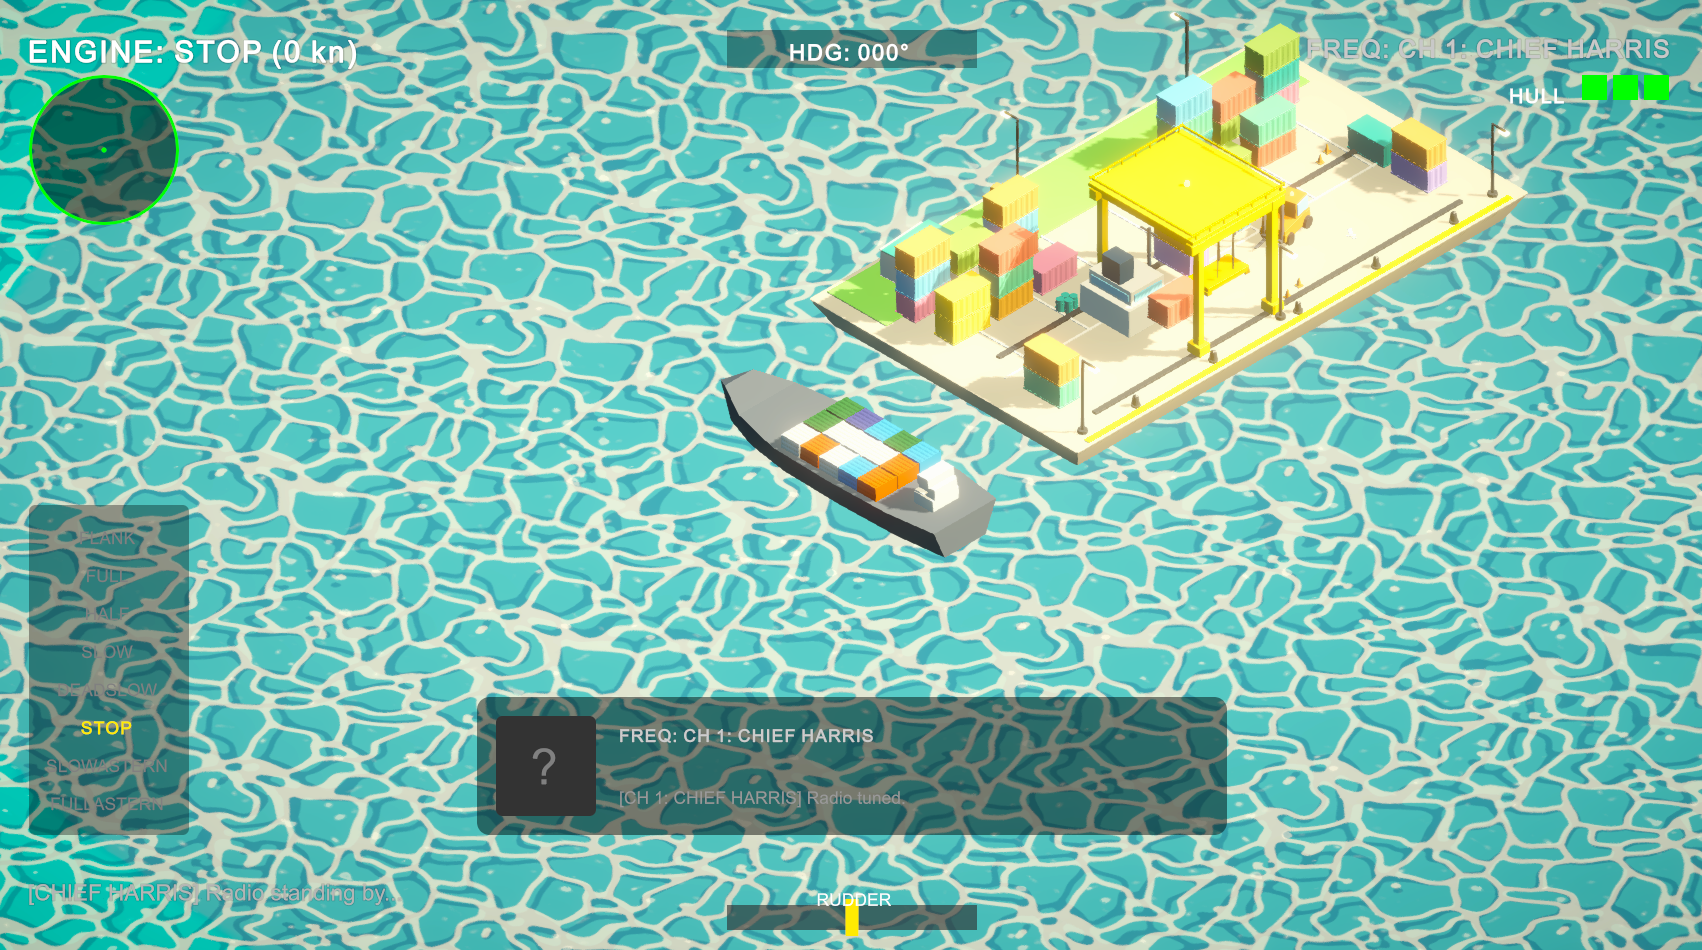
\includegraphics[width=\linewidth]{Document/GameDev/images/StartUI.png}\vspace{0.1cm} & 
\textbf{ฉากที่ 1: การรับมอบหมายภารกิจ}\newline
ผู้เล่นเริ่มต้นเกมในฐานะกัปตันเรือ หน้าจอแสดงบรรยากาศห้องบังคับการเรือ (Ship Bridge) พร้อมเสียงคลื่นและลมทะเล (Ambient Audio) เพื่อสร้างความรู้สึกดื่มด่ำ (Immersion) กัปตันได้รับมอบหมายให้นำเรือเดินทางไปยังจุดหมายปลายทางอย่างปลอดภัย \\ \hline

\vspace{0.1cm}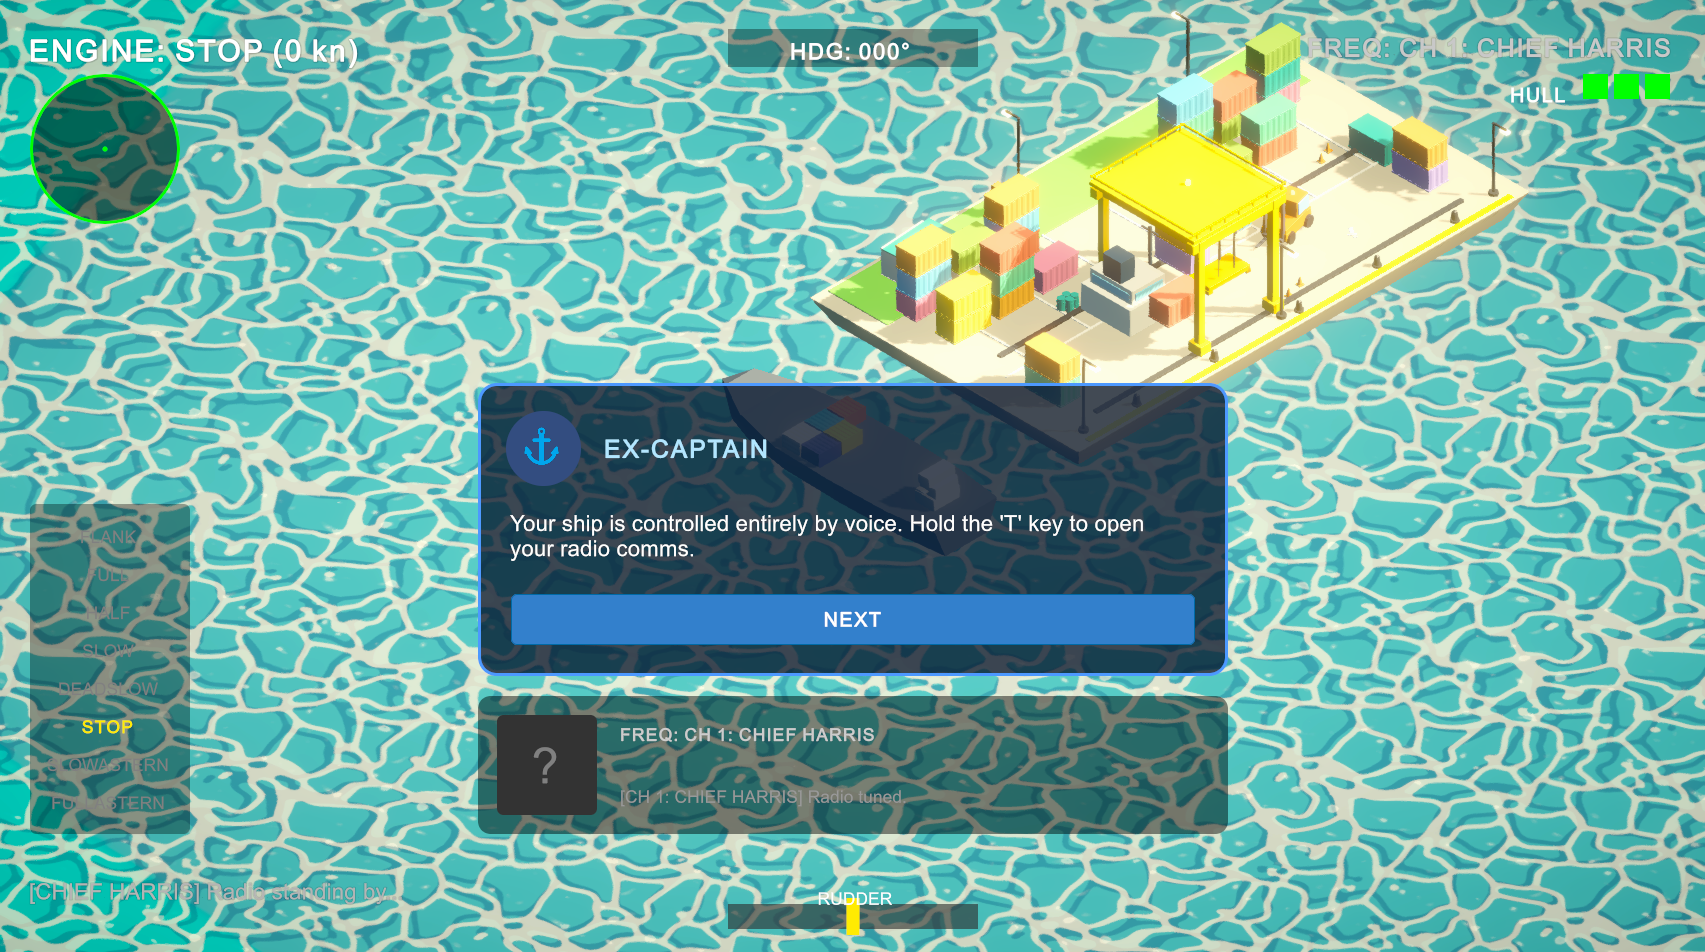
\includegraphics[width=\linewidth]{Document/GameDev/images/Tutorial.png}\vspace{0.1cm} &
\textbf{ฉากที่ 2: การแนะนำลูกเรือปัญญาประดิษฐ์}\newline
แนะนำตัวละครลูกเรือ AI สองตำแหน่ง ได้แก่ พลต้นหนผู้คอยแจ้งเตือนภัยจากเรดาร์ และพลถือท้ายผู้รอรับคำสั่งพวงมาลัย เกมเริ่มเข้าสู่โหมดการฝึกสอน (Tutorial) การออกคำสั่งเสียงภาษาอังกฤษพื้นฐาน \\ \hline

\vspace{0.1cm}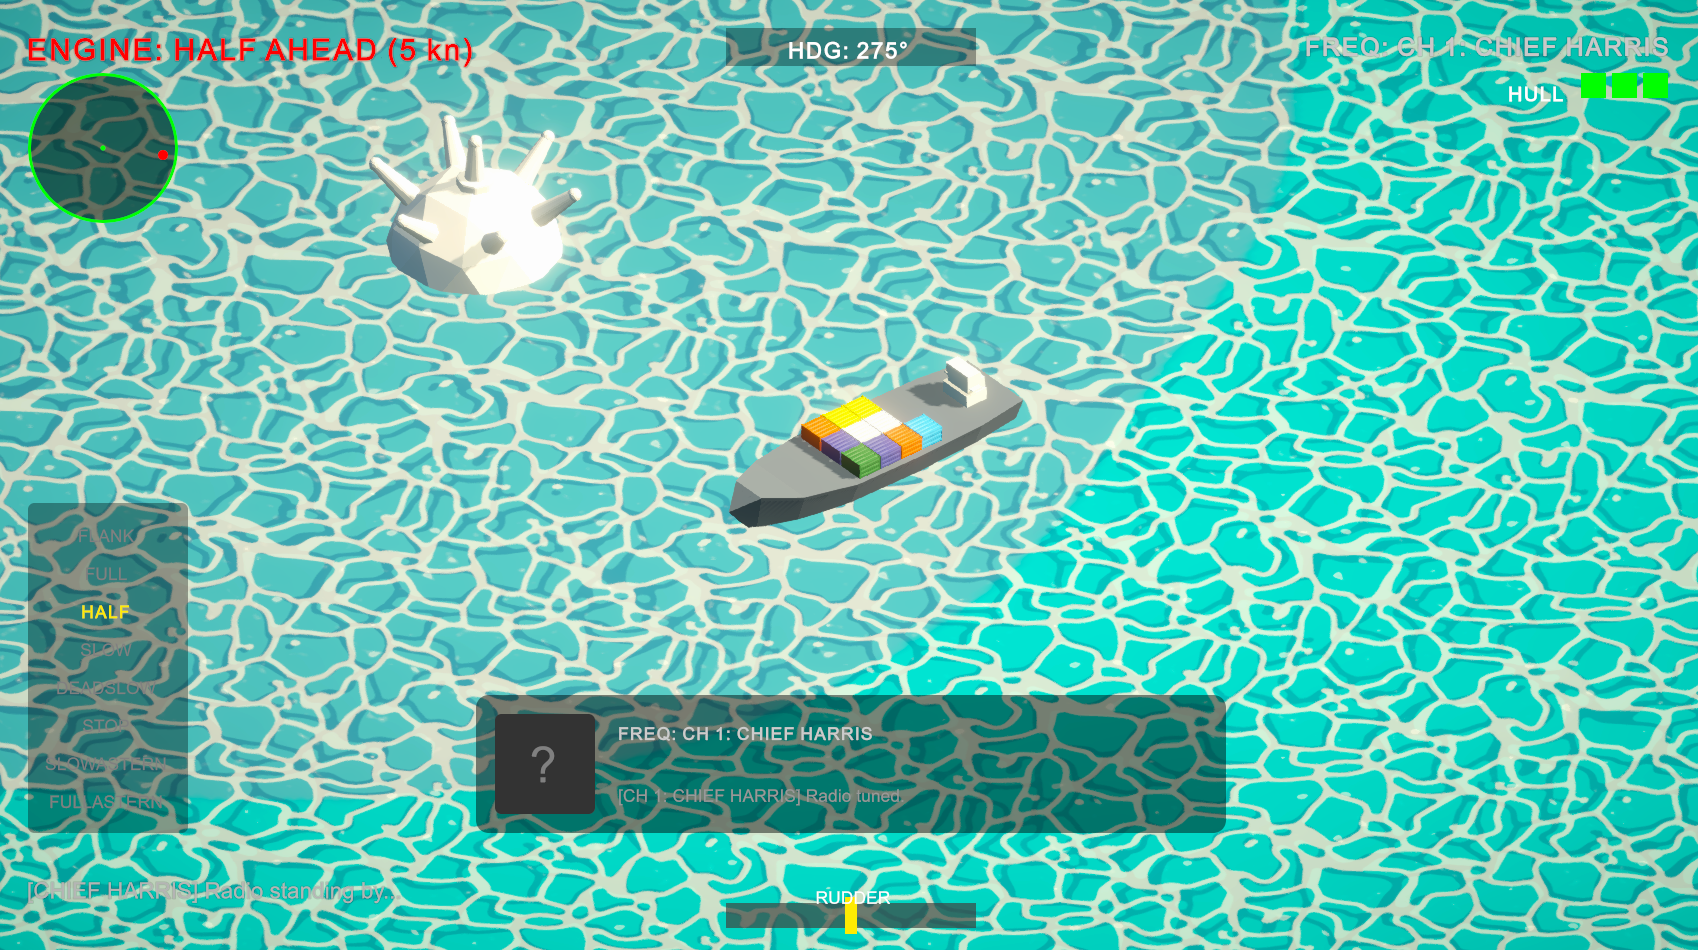
\includegraphics[width=\linewidth]{Document/GameDev/images/Hazard.png}\vspace{0.1cm} &
\textbf{ฉากที่ 3: สถานการณ์เผชิญหน้าสิ่งกีดขวาง}\newline
ระบบสุ่มสร้างอุปสรรค เช่น โขดหินหรือเรือลำอื่นขวางหน้า เรดาร์ส่งสัญญาณเตือนภัย ผู้เล่นต้องรีบประเมินสถานการณ์และเปล่งเสียงสั่งการแบบฉุกเฉินภายในเวลาที่กำหนด \\ \hline

\vspace{0.1cm}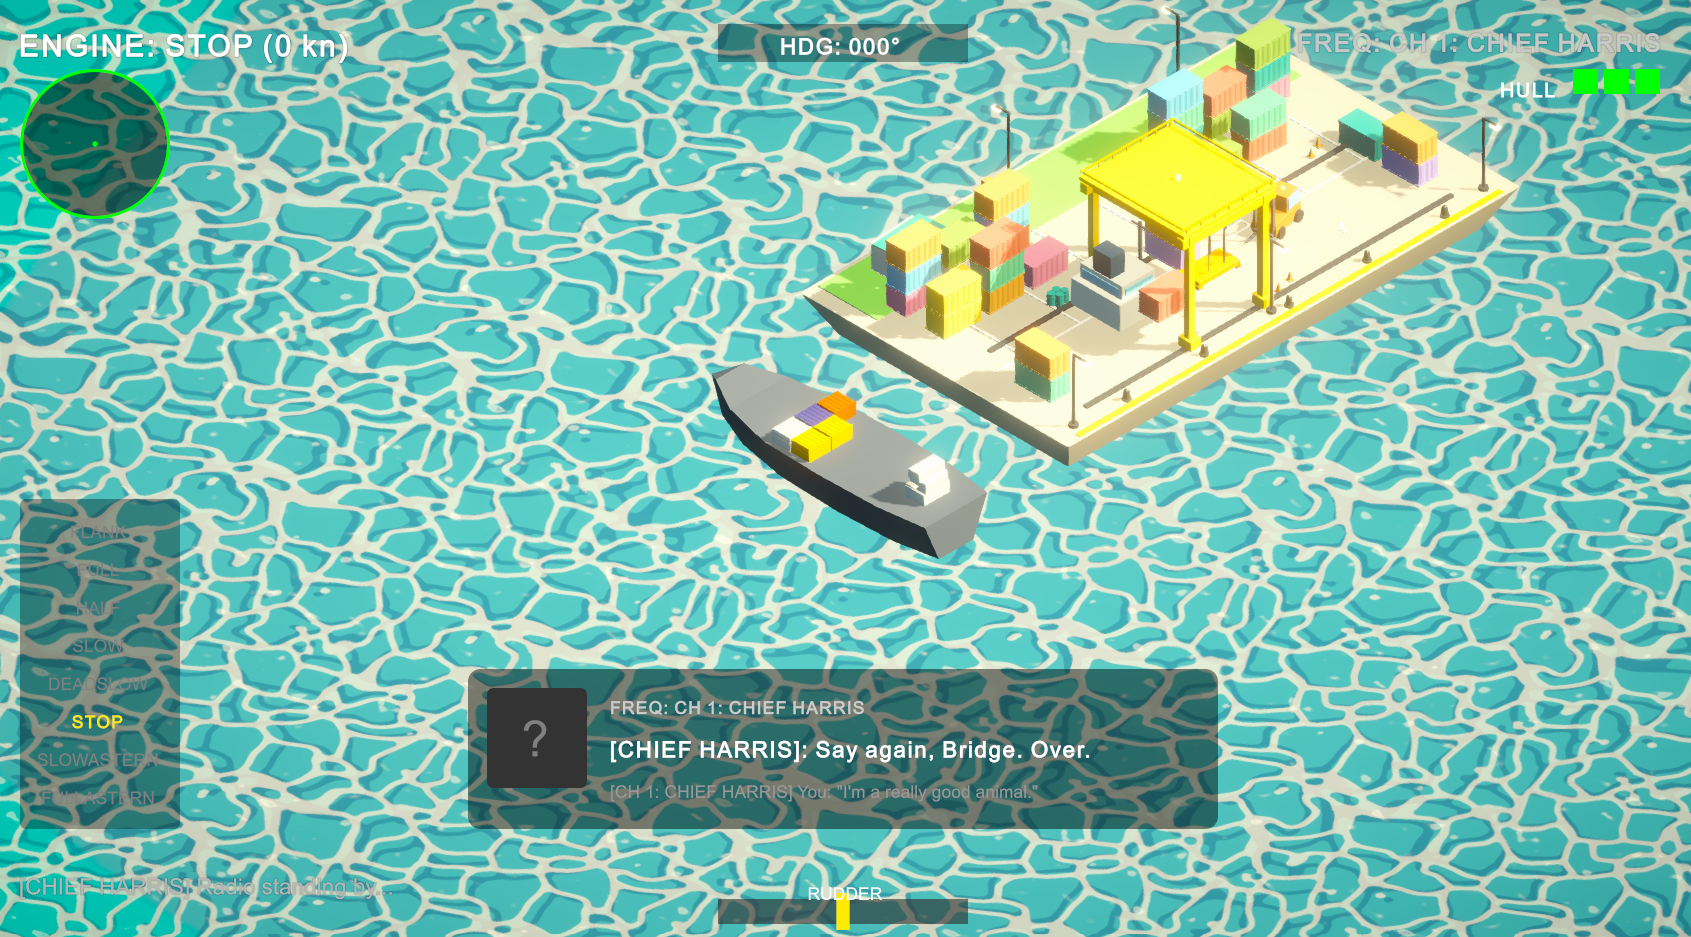
\includegraphics[width=\linewidth]{Document/GameDev/images/Sayagain.png}\vspace{0.1cm} & 
\textbf{ฉากที่ 4: สถานการณ์สื่อสารติดขัด (Clarification Request)}\newline
หากผู้เล่นออกเสียงไม่ชัดเจนหรือใช้คำสั่งผิดพลาด ลูกเรือ AI จะจำลองสถานการณ์สื่อสารติดขัดและทวนถาม เช่น \textit{``Say again, Captain?''} เพื่อกระตุ้นให้ผู้เล่นฝึกการแก้ปัญหาและเปล่งเสียงให้ชัดเจนขึ้น \\ \hline

\vspace{0.1cm}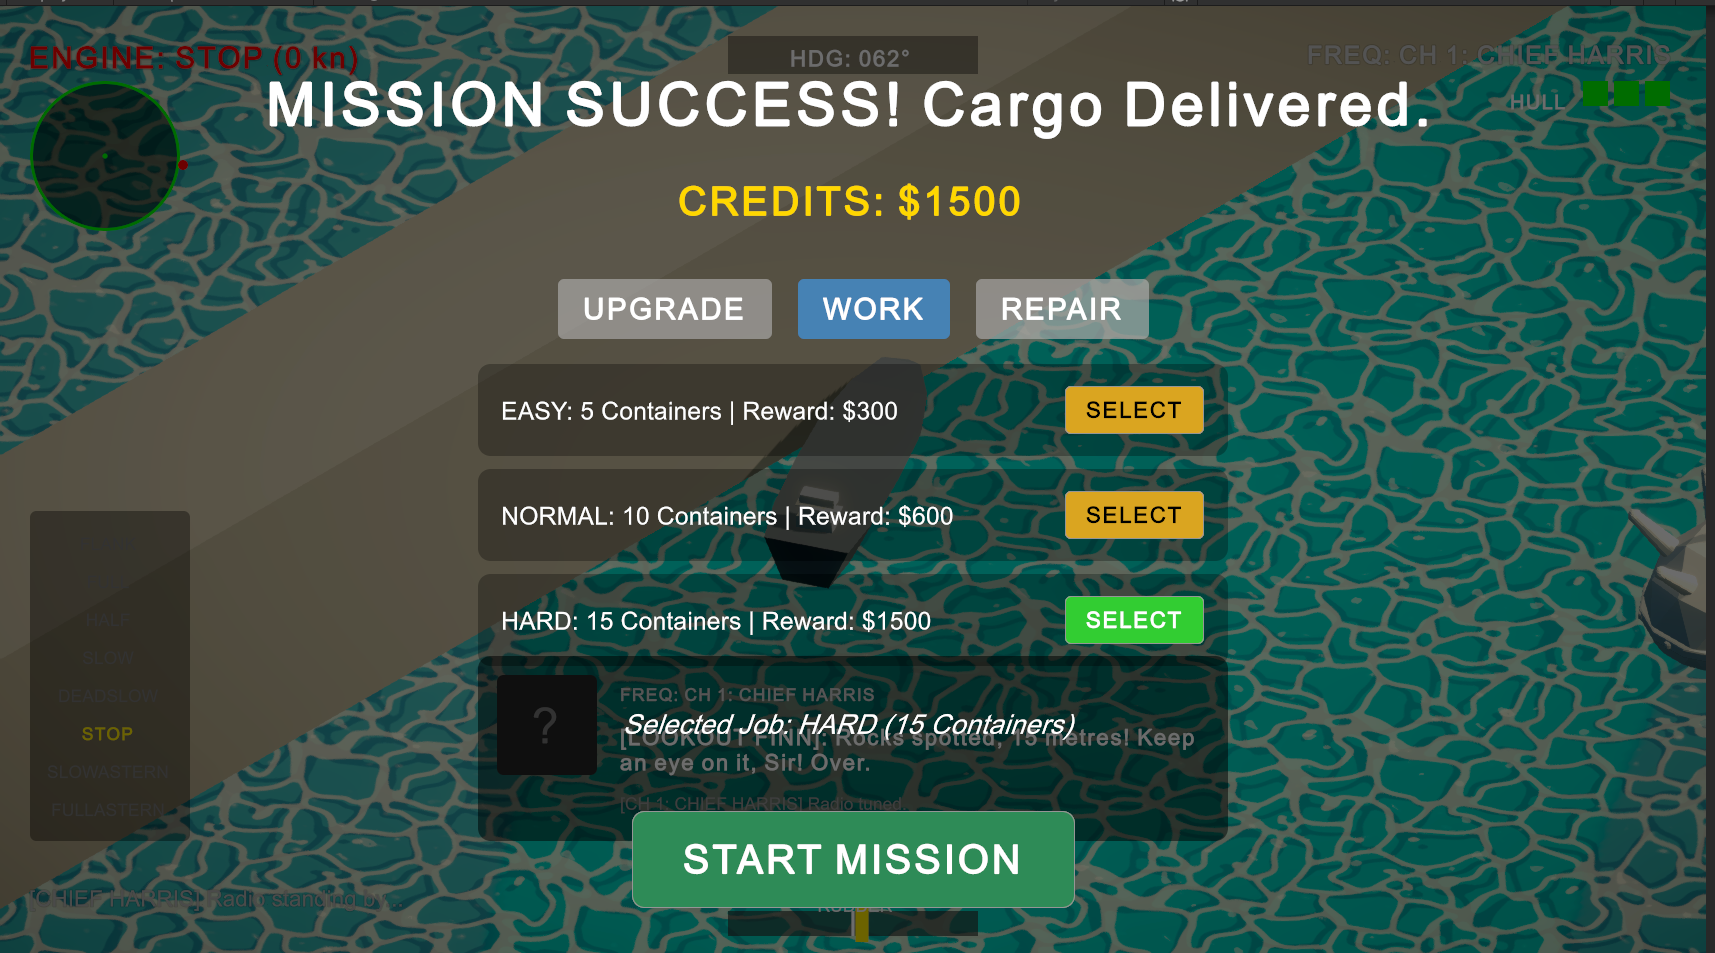
\includegraphics[width=\linewidth]{Document/GameDev/images/Victory.png}\vspace{0.1cm} & 
\textbf{ฉากที่ 5: สรุปผลภารกิจ (Result Screen)}\newline
หากนำเรือถึงเป้าหมายสำเร็จจะแสดงหน้าจอ Victory พร้อมสรุปคะแนนความแม่นยำในการออกเสียง แต่หากชนสิ่งกีดขวางจนมาตรวัดความเสียหายหมดลง จะแสดงหน้าจอ Game Over และต้องเริ่มภารกิจใหม่ \\
\hline
\end{tabular}
\end{table}